\subsection{Overview}
\begin{frame}
    
    \begin{itemize}
        \item VERA Progression Problems \cite{VERAProgressionProblems}
        \begin{itemize}
            \item Series of 10 benchmark problems based on Watts Bar Unit 1 Pressurized Water Reactor (PWR)
            \item Problems 4 and 5 were used to test polynomial and subplane CP methods
            \item Subray MOC was not used on these problems due to cross sections shielding requirements
        \end{itemize}
        \item C5G7 Benchmark Problems \cite{EELewisC5G72003,EELewisC5G7extended2005}
        \begin{itemize}
            \item Benchmark problem with UO$_2$ and MOX fuels
            \item 7 energy groups
            \item Various C5G7 configurations were used to test subray MOC and compare it to subplane CP
        \end{itemize}
    \end{itemize}

\end{frame}

%%%%%%%%%%%%%%%%%%%%%%%%%%%%%%%%%%%%%%%%%%%%%%%%%%%%%%%%%%%%%%%%%%%%%%%%%%%%%%%%

\subsection{VERA Problem 4}
\begin{frame}[t]{Problem Description}
    
\begin{columns}
    \begin{column}{0.5\textwidth}
        \begin{itemize}
            \item Center 3x3 assembly cluster in Watts Bar Unit 1
            \item AIC control rod in center assembly placed at 257.9 cm
            \item Test cases used 57 planes, with rod inserted 50\% into a plane
            \item Reference used 58 planes, with extra plane boundary aligned 
            with rod tip
            \item All simulations used 1 core per plane
        \end{itemize}
    \end{column}
    \begin{column}{0.28\textwidth}
        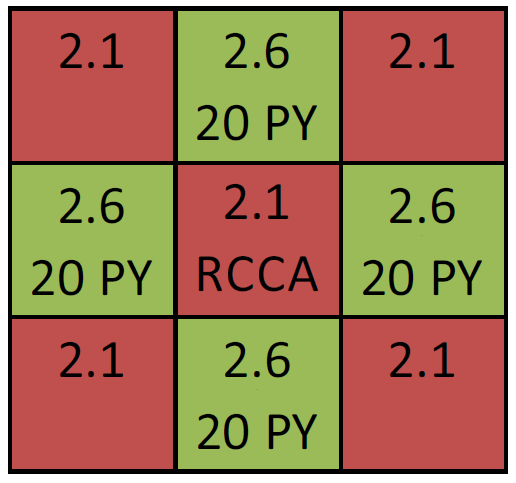
\includegraphics[width=\textwidth]{p4a_layout.png}
    \end{column}
    \begin{column}{0.22\textwidth}
        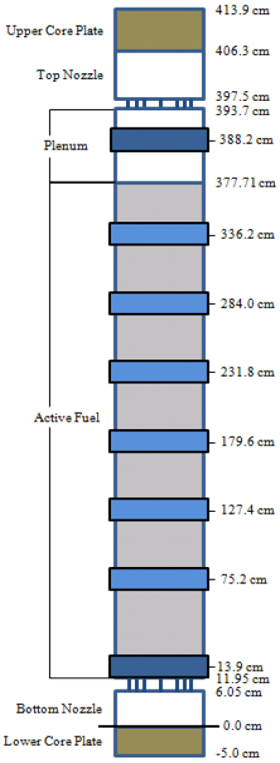
\includegraphics[width=\textwidth]{wb_3d_assembly.png}
\end{column}
\end{columns}
    
\end{frame}

%%%%%%%%%%%%%%%%%%%%%%%%%%%%%%%%%%%%%%%%%%%%%%%%%%%%%%%%%%%%%%%%%%%%%%%%%%%%%%%%%

\begin{frame}[t]{Test Procedures}
    
    \begin{itemize}
        \item Differential rod worth curves were generated with fine mesh, coarse mesh, and each decusping method
        \item Comparison of curves shows effectiveness of decusping methods as rod is withdrawn through core
        \item KENO-VI was used to calculate reference solutions at 10\% intervals
        \begin{itemize}
            \item 500 inactive generations (Need to update keno comparisons)
            \item 10,000 active generations
            \item $5\times 10^6$ particles per generation
        \end{itemize}
    \end{itemize}

\end{frame}

%%%%%%%%%%%%%%%%%%%%%%%%%%%%%%%%%%%%%%%%%%%%%%%%%%%%%%%%%%%%%%%%%%%%%%%%%%%%%%%%%

\begin{frame}[t]{Differential Rod Worth Curve}
    
\begin{center}
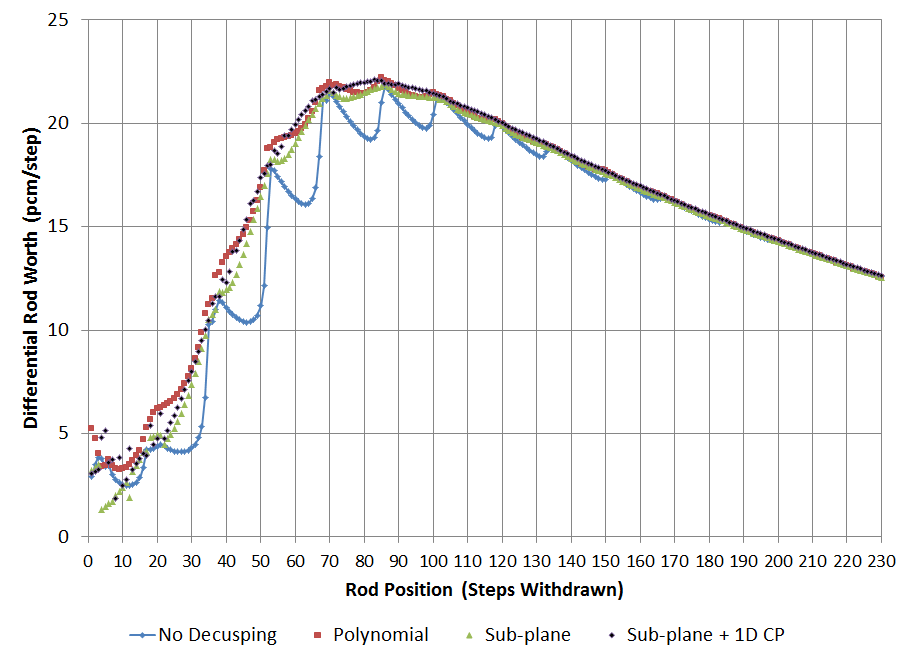
\includegraphics[width=0.8\textwidth]{differentialRodworth.png}
\end{center}
    
\end{frame}

%%%%%%%%%%%%%%%%%%%%%%%%%%%%%%%%%%%%%%%%%%%%%%%%%%%%%%%%%%%%%%%%%%%%%%%%%%%%%%%%%

\begin{frame}[t]{KENO-VI Comparisons}
    
    \vspace{-20pt}
    \begin{table}[h]
        \sisetup{separate-uncertainty=true,table-text-alignment=left,table-number-alignment=left}
        \resizebox{\textwidth}{!}{\begin{tabular}{l l 
                S[table-format=3.1,table-number-alignment=left] 
                S[table-format=1.3,table-number-alignment=left] 
                S[table-format=2.3,table-number-alignment=left]}\toprule
            \multirow{2}{*}{Cases} & \multirow{2}{*}{{Decusping Method}} & \multirow{2}{*}{{\keff{} 
                    Difference}} & 
            \multicolumn{2}{l}{{Pin Power Difference}} \\
            &  &  & {RMS} & {Max} \\\midrule
            \multirow{4}{*}{Average}       & None              &   -17.7 &  4.833\% & 23.037\% \\
            & Polynomial        &    35.5 &  1.365\% &  8.003\% \\
            & Subplane          &    35.5 &  0.940\% &  4.210\% \\
            & Subplane + CP     &    41.5 &  0.730\% &  3.069\% 
            \\\midrule
            \multirow{2}{*}{Worst -- 20\%} & None              & -174.5 & 14.893\% & 63.700\% \\
            & Polynomial        & 15.4   &  3.492\% & 25.145\% \\
            & Subplane          & 11.1   &  2.089\% & 10.096\% \\
            & Subplane + CP     & 47.4   &  1.143\% &  4.534\% \\
            \midrule
            Fully Withdrawn                & --                & 40.1   & 0.242\%   & 0.824\% \\
            \bottomrule
        \end{tabular}
    }
    \end{table}

    \begin{itemize}
        \item 10,000 active generations, $5\times 10^6$ particles per generation
        \item Maximum \keff{} uncertainty is 0.6 pcm
        \item Maximum pin power uncertainty anywhere is less than 0.002
    \end{itemize}
    
\end{frame}

%%%%%%%%%%%%%%%%%%%%%%%%%%%%%%%%%%%%%%%%%%%%%%%%%%%%%%%%%%%%%%%%%%%%%%%%%%%%%%%%%

\subsection{VERA Problem 5}
\begin{frame}[t]{Problem Description and Test Procedures}
    
    \vspace{-10pt}
    \begin{itemize}
      \item Bank D inserted to 257.9 cm, other banks all out
      \item 57 planes for tests and 58 for reference, 16 cores per plane
      \item Decusping methods compared with fine mesh solution
    \end{itemize}
    \begin{figure}[h]
      \centering
      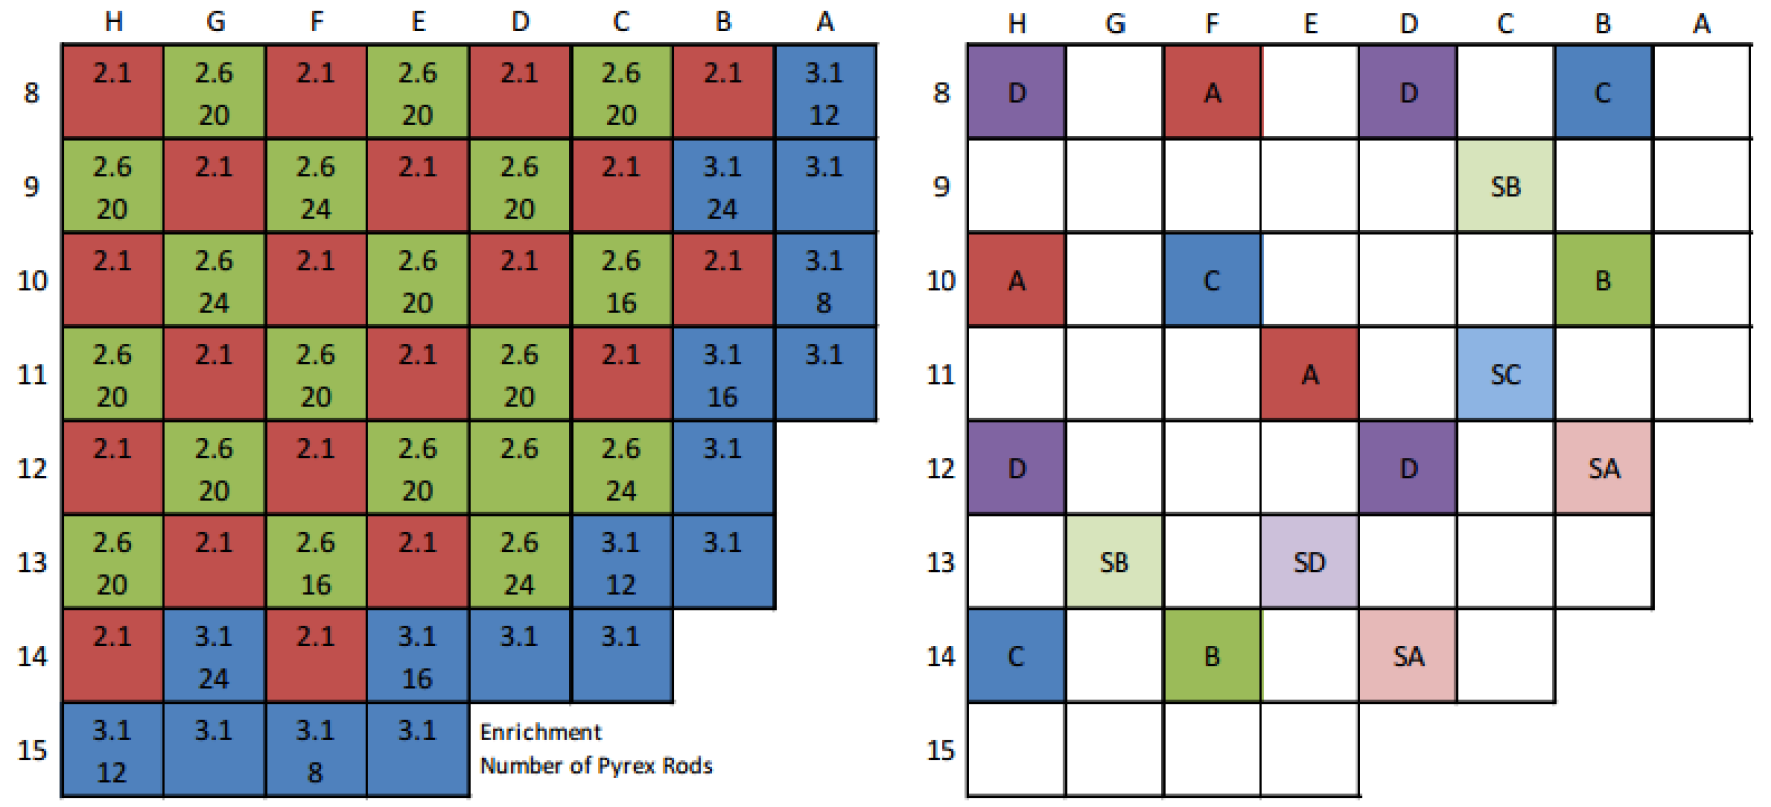
\includegraphics[width=0.9\textwidth]{WB1-cycle1-layout.png}
    \end{figure}
    
\end{frame}

%%%%%%%%%%%%%%%%%%%%%%%%%%%%%%%%%%%%%%%%%%%%%%%%%%%%%%%%%%%%%%%%%%%%%%%%%%%%%%%%%

\begin{frame}[t]{Problem 5 Results}
    
    \begin{table}[h]
      \centering
      \resizebox{\textwidth}{!}{
        \begin{tabular}{l c c S[table-format=2.2,table-number-alignment=left] c c c}\toprule
        \multirow{2}{*}{Case} & \keff{} & \multicolumn{2}{c}{{Pin Power Differences}} & \multicolumn{2}{c}{Iterations} & Runtime\\
        & Difference (pcm) & RMS & {Max} & 2D/1D & CMFD & (Core-Hours) \\\midrule
        Reference        &  -- & --     & {--}      & 13 & 481 & 361.7 \\
        No Treatment     & -22 & 6.90\% & 30.55\% & 13 & 523 & 410.7 \\
        Polynomial       &  -5 & 1.15\% &  4.85\% & 13 & 463 & 373.7 \\
        Subplane         &  -5 & 2.09\% & 10.20\% & 13 & 499 & 399.0 \\
        Subplane + CP    &  -1 & 0.50\% &  2.74\% & 13 & 529 & 425.6 \\
        \bottomrule
    \end{tabular}
      }
    \end{table}
    \begin{itemize}
        \item Maximum error for each comparison occurs in pins neighboring the partially rodded pin cell
    \end{itemize}
    
\end{frame}

%%%%%%%%%%%%%%%%%%%%%%%%%%%%%%%%%%%%%%%%%%%%%%%%%%%%%%%%%%%%%%%%%%%%%%%%%%%%%%%%

\subsection{2D C5G7}
\begin{frame}[t]{Problem Description}
 
\begin{columns}
\begin{column}{0.6\textwidth}
\vspace{-0.25in}
\begin{center}
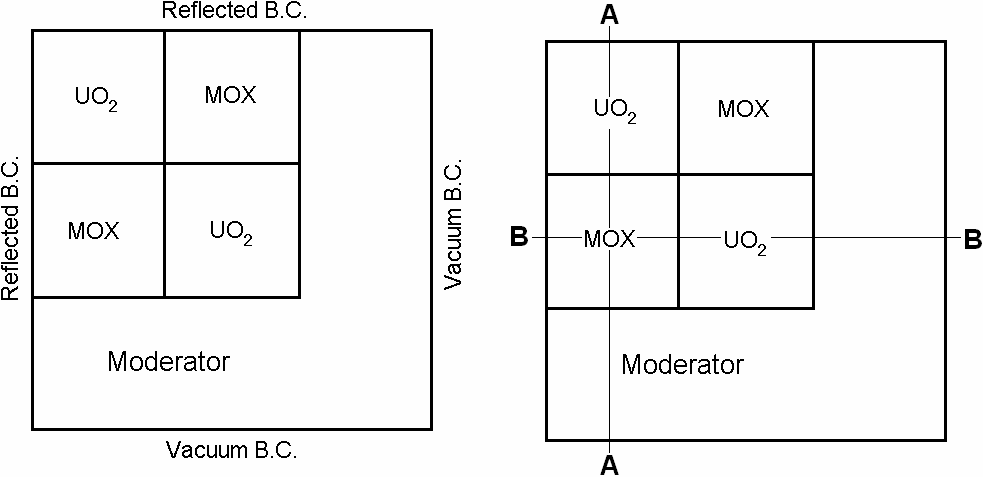
\includegraphics[width=\columnwidth]{c5g7-core-radial.png}

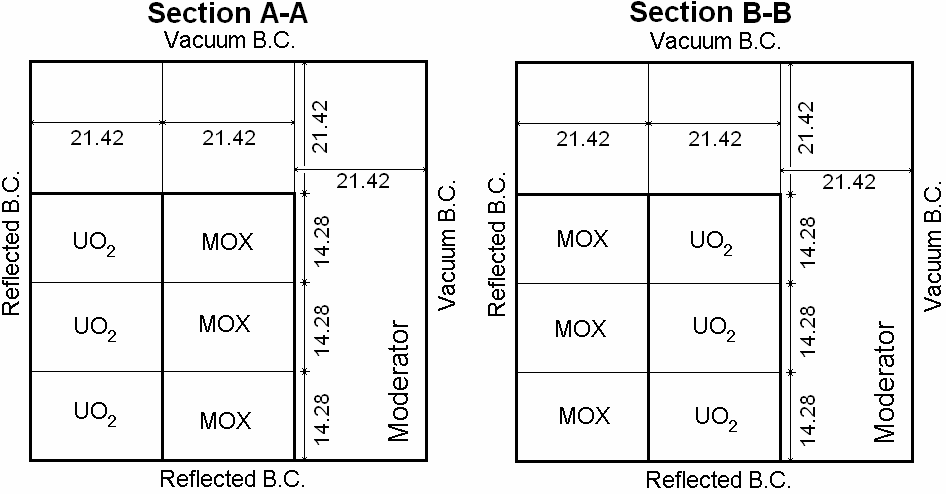
\includegraphics[width=\columnwidth]{c5g7-core-axial.png}
\end{center}
\end{column}
\begin{column}{0.4\textwidth}
    \begin{center}
    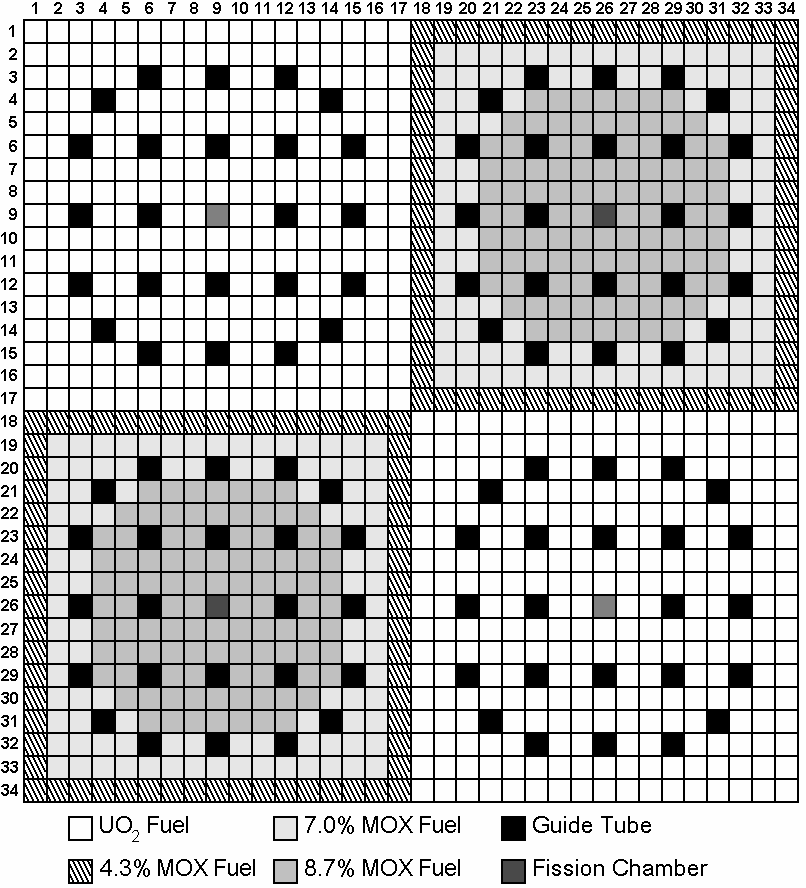
\includegraphics[width=\columnwidth]{c5g7-assemblies-radial.png}
\end{center}
\end{column}
\end{columns}
    
\end{frame}

%%%%%%%%%%%%%%%%%%%%%%%%%%%%%%%%%%%%%%%%%%%%%%%%%%%%%%%%%%%%%%%%%%%%%%%%%%%%%%%%

\begin{frame}[t]{Test Procedure}
    
    \begin{itemize}
        \item Three different C5G7 problems were simulated: 2D core, 3D assembly, and 3D core
        \item Rod was withdrawn through each problem in 1 cm increments for subray MOC and subplane methods
        \item \keff{} and 3D pin power comparisons were made against a fine mesh reference solution at each position
    \end{itemize}
    
\end{frame}

%%%%%%%%%%%%%%%%%%%%%%%%%%%%%%%%%%%%%%%%%%%%%%%%%%%%%%%%%%%%%%%%%%%%%%%%%%%%%%%%

\begin{frame}[t]{2D Core Results}

\begin{table}[h]
    \resizebox{\textwidth}{!}{
        \begin{tabular}{| l | l | l l l | l l l | l l l | l l l |}
            \hline
            Rod & Reference & \multicolumn{3}{c|}{Subray-0} & \multicolumn{3}{c|}{Subray-1} & \multicolumn{3}{c|}{Subray-2} & \multicolumn{3}{c|}{Subray-3} \\
            Position & \keff{} & \keff{} & \multicolumn{2}{l|}{Pin Powers} & \keff{} & \multicolumn{2}{l|}{Pin Powers} & \keff{} & \multicolumn{2}{l|}{Pin Powers} & \keff{} & \multicolumn{2}{l|}{Pin Powers} \\
            &  &  & RMS & Max &  & RMS & Max &  & RMS & Max &  & RMS & Max \\
            \hline
            1* & 1.06839 & -15  & 0.10\% & 0.29\% & -15  & 0.10\% & 0.29\% & -15  & 0.10\% & 0.29\% & -15  & 0.10\% & 0.29\% \\
            2 & 1.07746 & -33  & 0.22\% & 0.67\% & -34  & 0.22\% & 0.68\% & -34  & 0.22\% & 0.67\% & -34  & 0.22\% & 0.67\% \\
            3 & 1.08777 & -53  & 0.32\% & 1.03\% & -56  & 0.34\% & 1.07\% & -55  & 0.34\% & 1.06\% & -55  & 0.34\% & 1.06\% \\
            4 & 1.09919 & -72  & 0.41\% & 1.34\% & -78  & 0.45\% & 1.45\% & -78  & 0.45\% & 1.44\% & -78  & 0.45\% & 1.44\% \\
            5 & 1.11160 & -89  & 0.46\% & 1.53\% & -99  & 0.51\% & 1.69\% & -98  & 0.50\% & 1.66\% & -98  & 0.50\% & 1.66\% \\
            6 & 1.12495 & -102 & 0.49\% & 1.66\% & -115 & 0.55\% & 1.83\% & -115 & 0.54\% & 1.82\% & -115 & 0.54\% & 1.81\% \\
            7 & 1.13925 & -112 & 0.49\% & 1.70\% & -127 & 0.55\% & 1.88\% & -126 & 0.55\% & 1.87\% & -126 & 0.55\% & 1.86\% \\
            8 & 1.15469 & -117 & 0.47\% & 1.65\% & -133 & 0.53\% & 1.83\% & -132 & 0.53\% & 1.81\% & -132 & 0.52\% & 1.81\% \\
            9* & 1.17190 & -117 & 0.43\% & 1.50\% & -127 & 0.46\% & 1.61\% & -126 & 0.46\% & 1.60\% & -126 & 0.46\% & 1.60\% \\
            \hline
            Average & -- & 79 & 0.38\% & 1.26\% & 87 & 0.41\% & 1.37\% & 87 & 0.41\% & 1.36\% & 87 & 0.41\% & 1.36\% \\
            \hline
        \end{tabular}
    }
\end{table}

\begin{itemize}
    \item Superscript * denotes cases run with axial diffusion instead of P$_3$
\end{itemize}

\end{frame}

%%%%%%%%%%%%%%%%%%%%%%%%%%%%%%%%%%%%%%%%%%%%%%%%%%%%%%%%%%%%%%%%%%%%%%%%%%%%%%%%

\begin{frame}[t]{2D Core Results}

\begin{table}
    \centering
    \resizebox{\textwidth}{!}{
        \begin{tabular}{|l| l| l l l| l S[table-format=2.2,table-number-alignment=left] S[table-format=2.2,table-number-alignment=left]| l l l| l l l|}
            \hline
            Rod & Reference & \multicolumn{3}{c|}{Subray-0} & \multicolumn{3}{c|}{{None}} & \multicolumn{3}{c|}{Subplane} & \multicolumn{3}{c|}{Subplane + CP} \\
            Position & \keff{} & \keff{} & \multicolumn{2}{l|}{Pin Powers} & \keff{} & \multicolumn{2}{l|}{Pin Powers} & \keff{} & \multicolumn{2}{l|}{Pin Powers} & \keff{} & \multicolumn{2}{l|}{Pin Powers} \\
            &  &  & RMS & Max &  & {RMS} & {Max} &  & RMS & Max &  & RMS & Max \\
            \hline
            1* & 1.06839 & -15  & 0.10\% & 0.29\% & -286  & 1.73 \% & 4.47 \% & -87  & 0.52\% & 1.35\% & -169 & 0.99\% & 2.46\% \\
            2  & 1.07746 & -33  & 0.22\% & 0.67\% & -811  & 4.75 \% & 12.70\% & -198 & 1.13\% & 3.06\% & -174 & 0.97\% & 2.57\% \\
            3  & 1.08777 & -53  & 0.32\% & 1.03\% & -1369 & 7.71 \% & 21.30\% & -290 & 1.56\% & 4.42\% & -181 & 0.97\% & 2.70\% \\
            4  & 1.09919 & -72  & 0.41\% & 1.34\% & -1918 & 10.33\% & 29.42\% & -360 & 1.83\% & 5.35\% & -185 & 0.94\% & 2.75\% \\
            5  & 1.11160 & -89  & 0.46\% & 1.53\% & -2400 & 12.25\% & 36.00\% & -405 & 1.93\% & 5.84\% & -184 & 0.88\% & 2.68\% \\
            6  & 1.12495 & -102 & 0.49\% & 1.66\% & -2738 & 13.12\% & 39.83\% & -424 & 1.89\% & 5.89\% & -174 & 0.78\% & 2.47\% \\
            7  & 1.13925 & -112 & 0.49\% & 1.70\% & -2820 & 12.55\% & 39.38\% & -416 & 1.72\% & 5.52\% & -155 & 0.65\% & 2.11\% \\
            8  & 1.15469 & -117 & 0.47\% & 1.65\% & -2478 & 10.08\% & 32.80\% & -377 & 1.44\% & 4.76\% & -124 & 0.48\% & 1.62\% \\
            9* & 1.17190 & -117 & 0.43\% & 1.50\% & -1461 & 5.31 \% & 18.00\% & -300 & 1.06\% & 3.60\% & -80  & 0.29\% & 1.00\% \\
            \hline
            Average & -- & 79 & 0.38\% & 1.26\% & 1809 & 8.65\% & 25.99\% & 317 & 1.45\% & 4.42\% & 158 & 0.77\% & 2.26\% \\
            \hline
        \end{tabular}
    }
\end{table}

\begin{itemize}
\item Superscript * denotes cases run with axial diffusion instead of P$_3$
\end{itemize}

\end{frame}

%%%%%%%%%%%%%%%%%%%%%%%%%%%%%%%%%%%%%%%%%%%%%%%%%%%%%%%%%%%%%%%%%%%%%%%%%%%%%%%%

\subsection{3D C5G7}
\begin{frame}[t]{3D Assembly Results}

\begin{table}[h]
    \resizebox{!}{0.25\textwidth}{\begin{tabular}{l l l l S[table-format=2.2,table-number-alignment=left]}\toprule
        \multirow{2}{*}{Case} & \multirow{2}{*}{Method} & \keff{} & \multicolumn{2}{l}{{Pin Powers}} \\
        &  & Diff. & RMS & {Max} \\\midrule
        \multirow{7}{*}{Average} & None        & 2193 & 6.05\% & 10.95\% \\
        & Subplane    & 222  & 0.88\% &  1.64\% \\
        & Subplane+CP & 114  & 0.45\% &  0.84\% \\
        & Subray-0    & 52   & 0.25\% &  0.54\% \\
        & Subray-1    & 56   & 0.25\% &  0.55\% \\
        & Subray-2    & 56   & 0.25\% &  0.54\% \\
        & Subray-3    & 56   & 0.25\% &  0.54\% \\
        \midrule
        \multirow{7}{*}{Position 8} & None          & -91 & 2.88\% & 4.19\% \\
        & Subplane      & -319  & 1.51\% & 2.66\% \\
        & Subplane + CP & -106 & 0.52\% & 0.89\% \\
        & Subray-0      & -104 & 0.53\% & 0.94\% \\
        & Subray-1      & -104 & 0.52\% & 0.94\% \\
        & Subray-2      & -105 & 0.53\% & 0.98\% \\
        & Subray-3      & -105 & 0.53\% & 0.98\% \\
        \bottomrule
    \end{tabular}
}
\end{table}

\end{frame}

%%%%%%%%%%%%%%%%%%%%%%%%%%%%%%%%%%%%%%%%%%%%%%%%%%%%%%%%%%%%%%%%%%%%%%%%%%%%%%%%

\begin{frame}[t]{3D Assembly Results}
    
    \begin{center}
        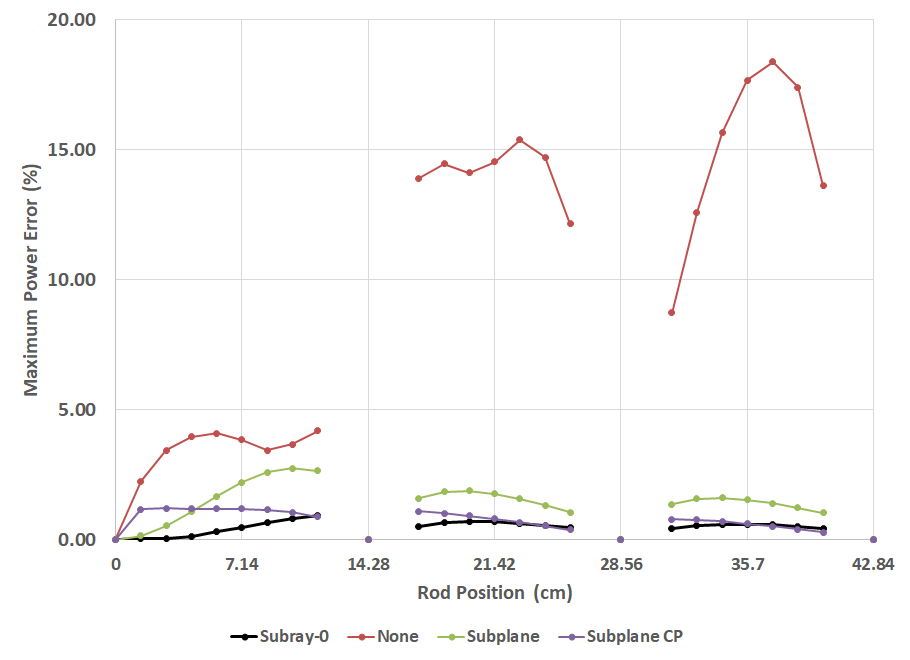
\includegraphics[width=0.8\textwidth]{subray-3dassem-errors.png}
    \end{center}
    
\end{frame}

%%%%%%%%%%%%%%%%%%%%%%%%%%%%%%%%%%%%%%%%%%%%%%%%%%%%%%%%%%%%%%%%%%%%%%%%%%%%%%%%

\begin{frame}[t]{3D Core Results}

\begin{table}[h]
    \resizebox{!}{0.25\textwidth}{\begin{tabular}{l l l S[table-format=2.2,table-number-alignment=left] S[table-format=2.2,table-number-alignment=left]}\toprule
        \multirow{2}{*}{Case} & \multirow{2}{*}{Method} & \keff{} & \multicolumn{2}{l}{{Pin Powers}} \\
        & & Diff. & {RMS} & {Max} \\\midrule
        \multirow{7}{*}{Average} & None        & 21 & 6.62\% & 29.30\% \\
        & Subplane    & 21 & 0.69\% & 3.47 \% \\
        & Subplane+CP & 21 & 0.34\% & 1.69 \% \\
        & Subray-0    & 21 & 0.20\% & 1.06 \% \\
        & Subray-1    & 25 & 0.20\% & 1.14 \% \\
        & Subray-2    & 25 & 0.20\% & 1.11 \% \\
        & Subray-3    & 21 & 0.20\% & 1.11 \% \\
        \midrule
        \multirow{7}{*}{Position 16} & None          & -1730 & 12.62\% & 55.69\% \\
        & Subplane      & -183 & 1.08\% & 5.61\% \\
        & Subplane + CP & -76 & 0.45\% & 2.38\% \\
        & Subray-0      & -46 & 0.30\% & 1.76\% \\
        & Subray-1      & -54 & 0.35\% & 2.01\% \\
        & Subray-2      & -53 & 0.34\% & 1.97\% \\
        & Subray-3      & -53 & 0.34\% & 1.96\% \\
        \bottomrule
    \end{tabular}
}
\end{table}

\end{frame}

%%%%%%%%%%%%%%%%%%%%%%%%%%%%%%%%%%%%%%%%%%%%%%%%%%%%%%%%%%%%%%%%%%%%%%%%%%%%%%%%

\begin{frame}[t]{3D Core Results}

\begin{center}
    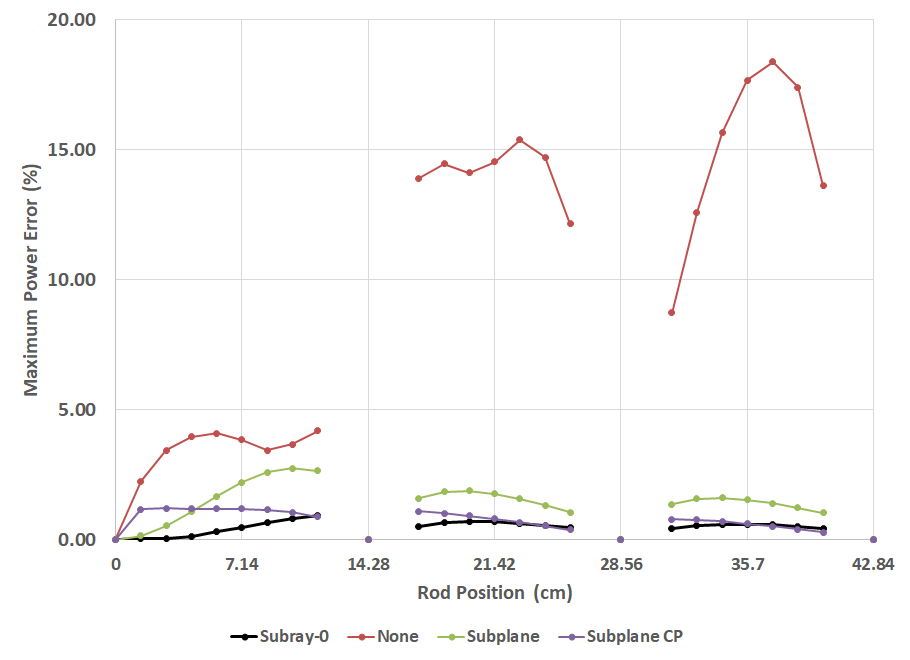
\includegraphics[width=0.8\textwidth]{subray-3dcore-errors.png}
\end{center}

\end{frame}